    %
% Credit to Tibault Reveyrand for the initial template - https://www.overleaf.com/articles/ieee-journal-submission-trans-on-mtt-example/pbfcbcjvmvmn

% ================================================
% Please HIGHLIGHT the new inputs such like this :
% Text :
%  \hl{comment}
% Aligned Eq. 
% \begin{shaded}
% \end{shaded}
% ================================================


\documentclass[journal]{IEEEtran}

%\usepackage[retainorgcmds]{IEEEtrantools}
%\usepackage{bibentry}  
\usepackage{xcolor,soul,framed} %,caption

\colorlet{shadecolor}{yellow}
% \usepackage{color,soul}
\usepackage[pdftex]{graphicx}
\graphicspath{{../images/}}
\DeclareGraphicsExtensions{.pdf,.jpeg,.png}

\usepackage[cmex10]{amsmath}
%Mathabx do not work on ScribTex => Removed
%\usepackage{mathabx}
\usepackage{array}
\usepackage{mdwmath}
\usepackage{mdwtab}
\usepackage{eqparbox}
\usepackage{url}

\hyphenation{op-tical net-works semi-conduc-tor}

%\bstctlcite{IEEE:BSTcontrol}


%=== TITLE & AUTHORS ====================================================================
\begin{document}
% \bstctlcite{IEEEexample:BSTcontrol}
    \title{Screening  Radiology  Images  for Lesion  Detection: An ML Approach}
  \author{Teodor~Ilie,~Jihyeon~Park,~and~Alex~Sun% <-this % stops a space

}  

% The paper headers
\markboth{}{}

% ====================================================================
\maketitle


% === 1. ABSTRACT ====================================================================
% =================================================================================
\begin{abstract}
%\boldmath
Radiologists manually evaluate large volumes of CT scans daily, and with this large workload comes the possibility of human error. Recent years have seen a rise in ``reckless-reading lawsuits", accusing radiologists of spending insufficient time viewing images, and leading to missed findings. At the same time, it is not unusual for experts to view images for only a second, and there is no clear research indicating that enforcing longer viewing times would improve accuracy; rather the issue is often with human error brought on by fatigue. \cite{workload}

Our primary aim is to improve the interpretation process by employing a state-of-the-art YOLOv3 image recognition model to give radiologists an additional tool to assist with their analysis, particularly for identifying lesions, which will improve patient diagnostic accuracy. Using the massive DeepLesion \cite{deeplesion} dataset, we train the model and determine its performance. Unfortunately, given the time constraint, we were unable to produce a model with sufficient accuracy for real-world use; additional work is required.

The output of the model can be deployed for use in hospitals, and be further inspected by radiologists to determine malignancy and subsequent treatment. We argue that such a tool improves the performance of human analysis alone, mitigating human error caused by fatigue, long hours, and other challenging circumstances radiologists face. 

We release the pre-processing and model PyTorch Jupyter code open-source for future research: \textit{\url{https://github.com/Aleyssu/DeepLesion-YOLOv3}} \end{abstract}

\begin{IEEEkeywords}
Radiology, DeepLesion, Convolutional Neural Network, U-Net, YOLO
\end{IEEEkeywords}


% === II. BACKGROUND =============================================================
% =================================================================================
\section{Background}
\subsection{CT Scans and Radiologist Workload}
% =======
% FIG. 01
% =======
% \begin{figure}
%  \begin{center}
%  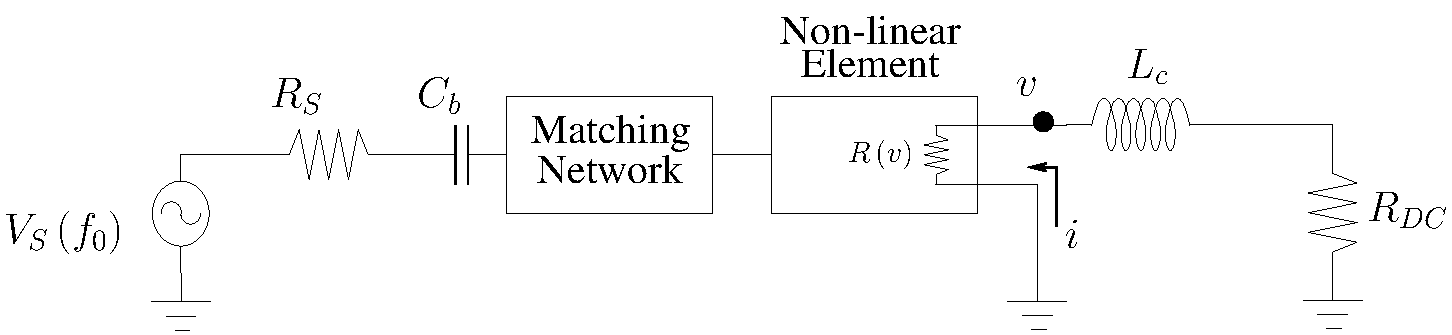
\includegraphics[width=3.5in]{pdf/01.pdf}\\
%  \caption{Caption}\label{circuit_diagram}
%  \end{center}
%\end{figure}

\IEEEPARstart{C}{omputed} Tomography (CT) scanners take many cross-sectional areas at fixed-length intervals along a specific body part, generating dozens or even hundreds of scans depending on the area of interest \cite{PMID:33620865}. There are many use cases for CT scans including preventative medicine and cancer screening, but scanning for lesions is particularly useful. A lesion is visible on a CT scan as it looks abnormal from the surrounding tissue, and radiologists manually inspect scans to determine parameters like the size and shape of the lesion. Lesions fall into several categories, including benign lesions such as cysts and fibromas, cancerous lesions such as tumours and metastases, and infectious lesions such as abscesses and granulomas. Lesion types cannot always be classified from CT scans alone, and subsequent tests such as biopsies, additional imaging tests such as MRI and ultrasound, blood tests, and others are used to determine the lesions cause and treatment courses \cite{oncology}.

% =======
% FIG. 01
% =======
\begin{figure}
 \begin{center}
 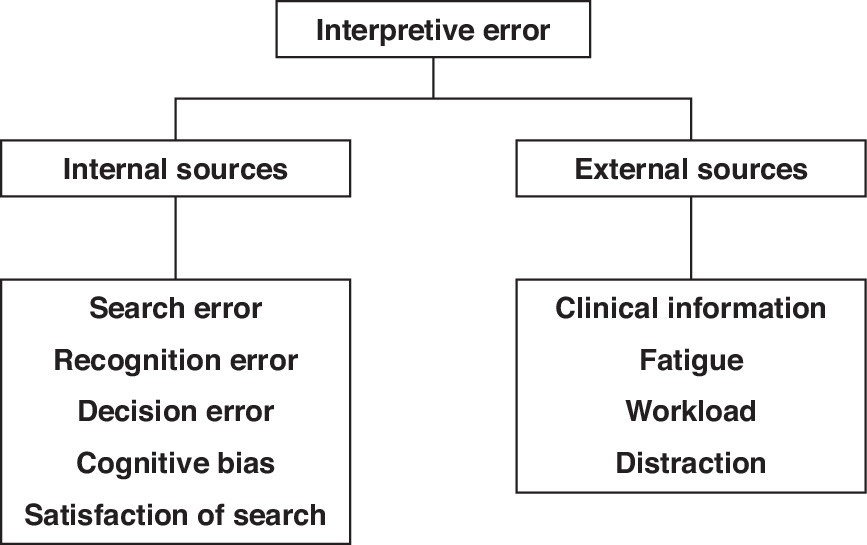
\includegraphics[width=2.5in]{images/scan_error.jpeg}\\
 \caption{Categories of interpretive error, both internal and external \cite{radiology_error}.}\label{interpret_error}
 \end{center}
\end{figure}

As the use of medical imaging such as CT scans continues to grow due to its numerous applications, radiologists are in increasing demand, yet expert radiologists are a scarce resource due to the time and challenges of training. This is placing increasing strain on the time and resources of existing radiologists, leading to climbing medical errors brought on by fatigue, and it is a leading cause of litigation. Medical error is a serious issue; Makary et al. have argued that should medical error, in general, be treated as a disease, it would rank as the third top cause of death in the US \cite{medical_error}. 

An overview of the most common ways radiologists are affected by interpretive error is given in Figure \ref{interpret_error}. Funaki et al. have determined that as much as 60-80\% of errors, depending on the context, are caused by perception error \cite{perception_error}. In addition, there has been a sevenfold increase in image interpretations performed per minute from 1999 to 2000, which is likely causing human errors to increase due to fatigue from the increased workload \cite{radiology_error}. 

At the same time, it is challenging to determine and implement meaningful workload limitations for radiologists, given the complexity of the process and the variation from person to person. While it is well-established that reducing the viewing time negatively affects interpretation accuracy, prescribing blanket variations for all radiologists would also be arbitrary and ineffective, as such regulations would not account for the varying degrees to which different people are affected by the same circumstances. As such, radiologists continue to self-regulate the workload to a great extent. Furthermore, external factors such as distraction and cognitive biases are even more challenging to address with regulation or training \cite{workload}. 

\subsection{Improvements through AI}
Many of these human errors have the potential to be dramatically improved through the use of computer-aided diagnosis, and in particular, modern AI image recognition models, aiding radiologists to make more accurate assessments that improve patient outcomes. With lesion detection being one of the most important yet time-consuming tasks of radiologists, such a tool would be immensely useful \cite{deep_learning_survey}. As these models continue to improve, they have already seen successful applications in providing radiologists with a second opinion in real-time, acting as a ``safety net". Of particular interest is the fact that they are entirely unaffected by human errors of bias and fatigue, and as algorithms continue to improve, their perceptual abilities begin to compete with that of even trained radiologists \cite{workload}. Some experts even go so far as to claim that radiologists will gradually be altogether replaced by better-performing, cheaper, and faster AI systems \cite{ai_foe}, while others maintain that radiologists will continue to play the central role, and AI tools will remain just that - an additional tool to enhance their work quality \cite{doctors_ftw}. Either way, the consensus is clearly in favour of the benefits of increasing the quality and roll-out of AI models for improved diagnostic accuracy and quality, and its potential to save lives \cite{consensus}\cite{ai_adoption}. 

Since the dawn of Convolutional Neural Networks, and the seminal handwriting recognition work done by Yann LeCun and Yoshua Bengio, machine learning algorithms have taken the world by storm in their amazing application in the field of image recognition \cite{cnn_lecun_bengio}. CNNs work by applying "convolution filters", small matrices of weights, across an input image to compute feature maps, detecting things such as corners or edges. These are sent through activation functions, such as ReLU, to introduce non-linearity, and then through pooling layers to reduce the spatial dimensions and reduce the computational power necessary, while aiming to preserve the information. Finally, as with all deep learning architectures, they are fed through various layers, where artificial neurons are connected either sparsely or densely. 

Many models have since been developed that build on this fundamental base. The YOLO (You Only Look Once) model, or subsequent versions such as YOLOv2 through YOLOv7, is a single-stage detector, and as such is very fast but sacrifices some accuracy \cite{yolo}. In particular, YOLOv3 is a real-time object detection algorithm, whose speed is attributed to its single forward pass through a CNN. Unlike two-stage detectors such as R-CNN it performs object localization and classification in one unified step, using a feature pyramid to handle different object sizes, grid division and anchor boxes to predict probability scores and bounding boxes, and a multi-part loss function to enhance accuracy.


% === III. HYPOTHESIS ========================
% =================================================================================
\section{Hypothesis}
Our primary aim is to apply YOLOv3 to generate bounding boxes for lesions on CT scan images, comparing performance to the ground truth. We hypothesize that it can perform on-par, or even exceed, expert analysis.

% === IV. METHODS ========================
% =================================================================================
\section{Methods}
\subsection{Dataset overview}

% =======
% FIG. 02
% =======
\begin{figure}
 \begin{center}
 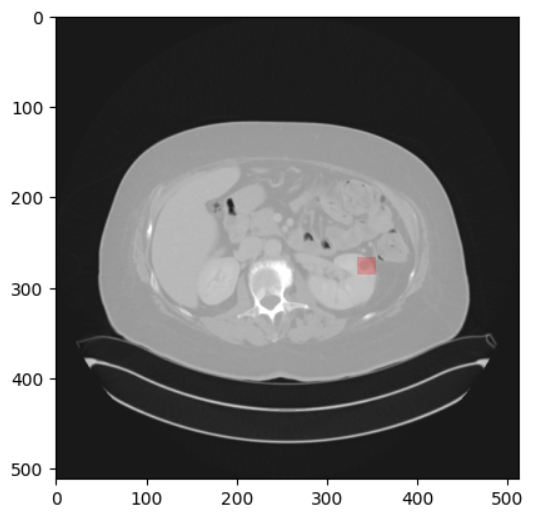
\includegraphics[width=2.5in]{images/example_scan.png}\\
 \caption{Example visualization of a DeepLesion scan, with lesion bounding box displayed in red}\label{example_scan}
 \end{center}
\end{figure}


The DeepLesion dataset contains 32,735 lesions in 32,120 CT slices from 10,594 studies of 4,427 unique patients \cite{deeplesion}, which is pre-filtered to remove faulty data. We train our model on a subset developed on Kaggle \cite{kaggle}. This dataset is publicly available and does not require special access permissions. The data is gathered from CT scan images that were annotated by radiologists during routine analysis, and stored as ``bookmarks" in hospitals' picture archiving and communication systems (PACS).  

Every image is annotated with a bounding box surrounding lesions, and each lesion contains information about the lesion diameter and lesion type. 

\subsection{Data pre-processing and model design}
We applied a version of the YOLOv3 model using the architecture developed by Redmon et al., to provide a fast diagnostic tool with minimal computational requirements to run \cite{yolov3}. This required data pre-processing to match the model's input requirements.

First, the images were read into an array using the PIL library, and then their values were converted from unsigned to signed format by subtracting 32768 \cite{deeplesion}. Most of the images in the dataset were 512x512 pixels in dimension, so the few that weren't were rescaled to 512x512. Afterwards, they were saved to a Pytorch tensor and split off into training, testing, and validation Pytorch dataset and dataloaders. Each image's corresponding bounding boxes were read from the CSV file and processed into a grid as labels for the model. As some scans were annotated with multiple bounding boxes corresponding to multiple lesions, multiple entries from the CSV were read in sequence to ensure all the bounding boxes for a given image were recorded.

Images were loaded into a visualizer to ensure bounding boxes were processed correctly. This would later be useful for converting the grids outputted by the YOLO model to bounding boxes, visualizing them, and comparing their performances to the ground truth bounding boxes. An example is shown in Figure \ref{example_scan}. 

The authors of YOLOv3 mention that attempting to directly predict bounding box coordinates with a linear activation in the final layer of the model worsens model stability and performance, so we added a sigmoid activation at the final layer \cite{yolov3}. As this normalized all the outputs to the range [0, 1], the labels had to be adjusted accordingly where 0 would represent the starting point and 1 the end point of all possible coordinate measurements.


% === V. RESULTS ========================
% =================================================================================
\section{Results}
We tested our model over a variety of different epochs to balance prediction accuracy with overfitting. The training and validation losses over the epochs are shown in Figure \ref{fig:compare}. As can be seen, training the model over 100 epochs led to a near-zero loss on the training set, but validation loss only went up. This is reflected on the testing set, where the model was unable to make any predictions (see Fig. \ref{fig:training} and Fig. \ref{fig:testing}). It is clear the model was being overfit and could not generalize to new images. At 50 epochs, the model made testing set predictions, but they were far off from the actual bounding boxes. We concluded that the model began to overfit before it was able to learn sufficient information to make predictions with high accuracy. It is possible that training on a larger subset or the entirety of the DeepLesion dataset would reduce overfitting and improve generalization, but time constraints and the computational limits of using a single personal computer to train the model with prevented us from attempting this.


% =======
% FIG. 03
% =======
\begin{figure}
 \begin{center}
 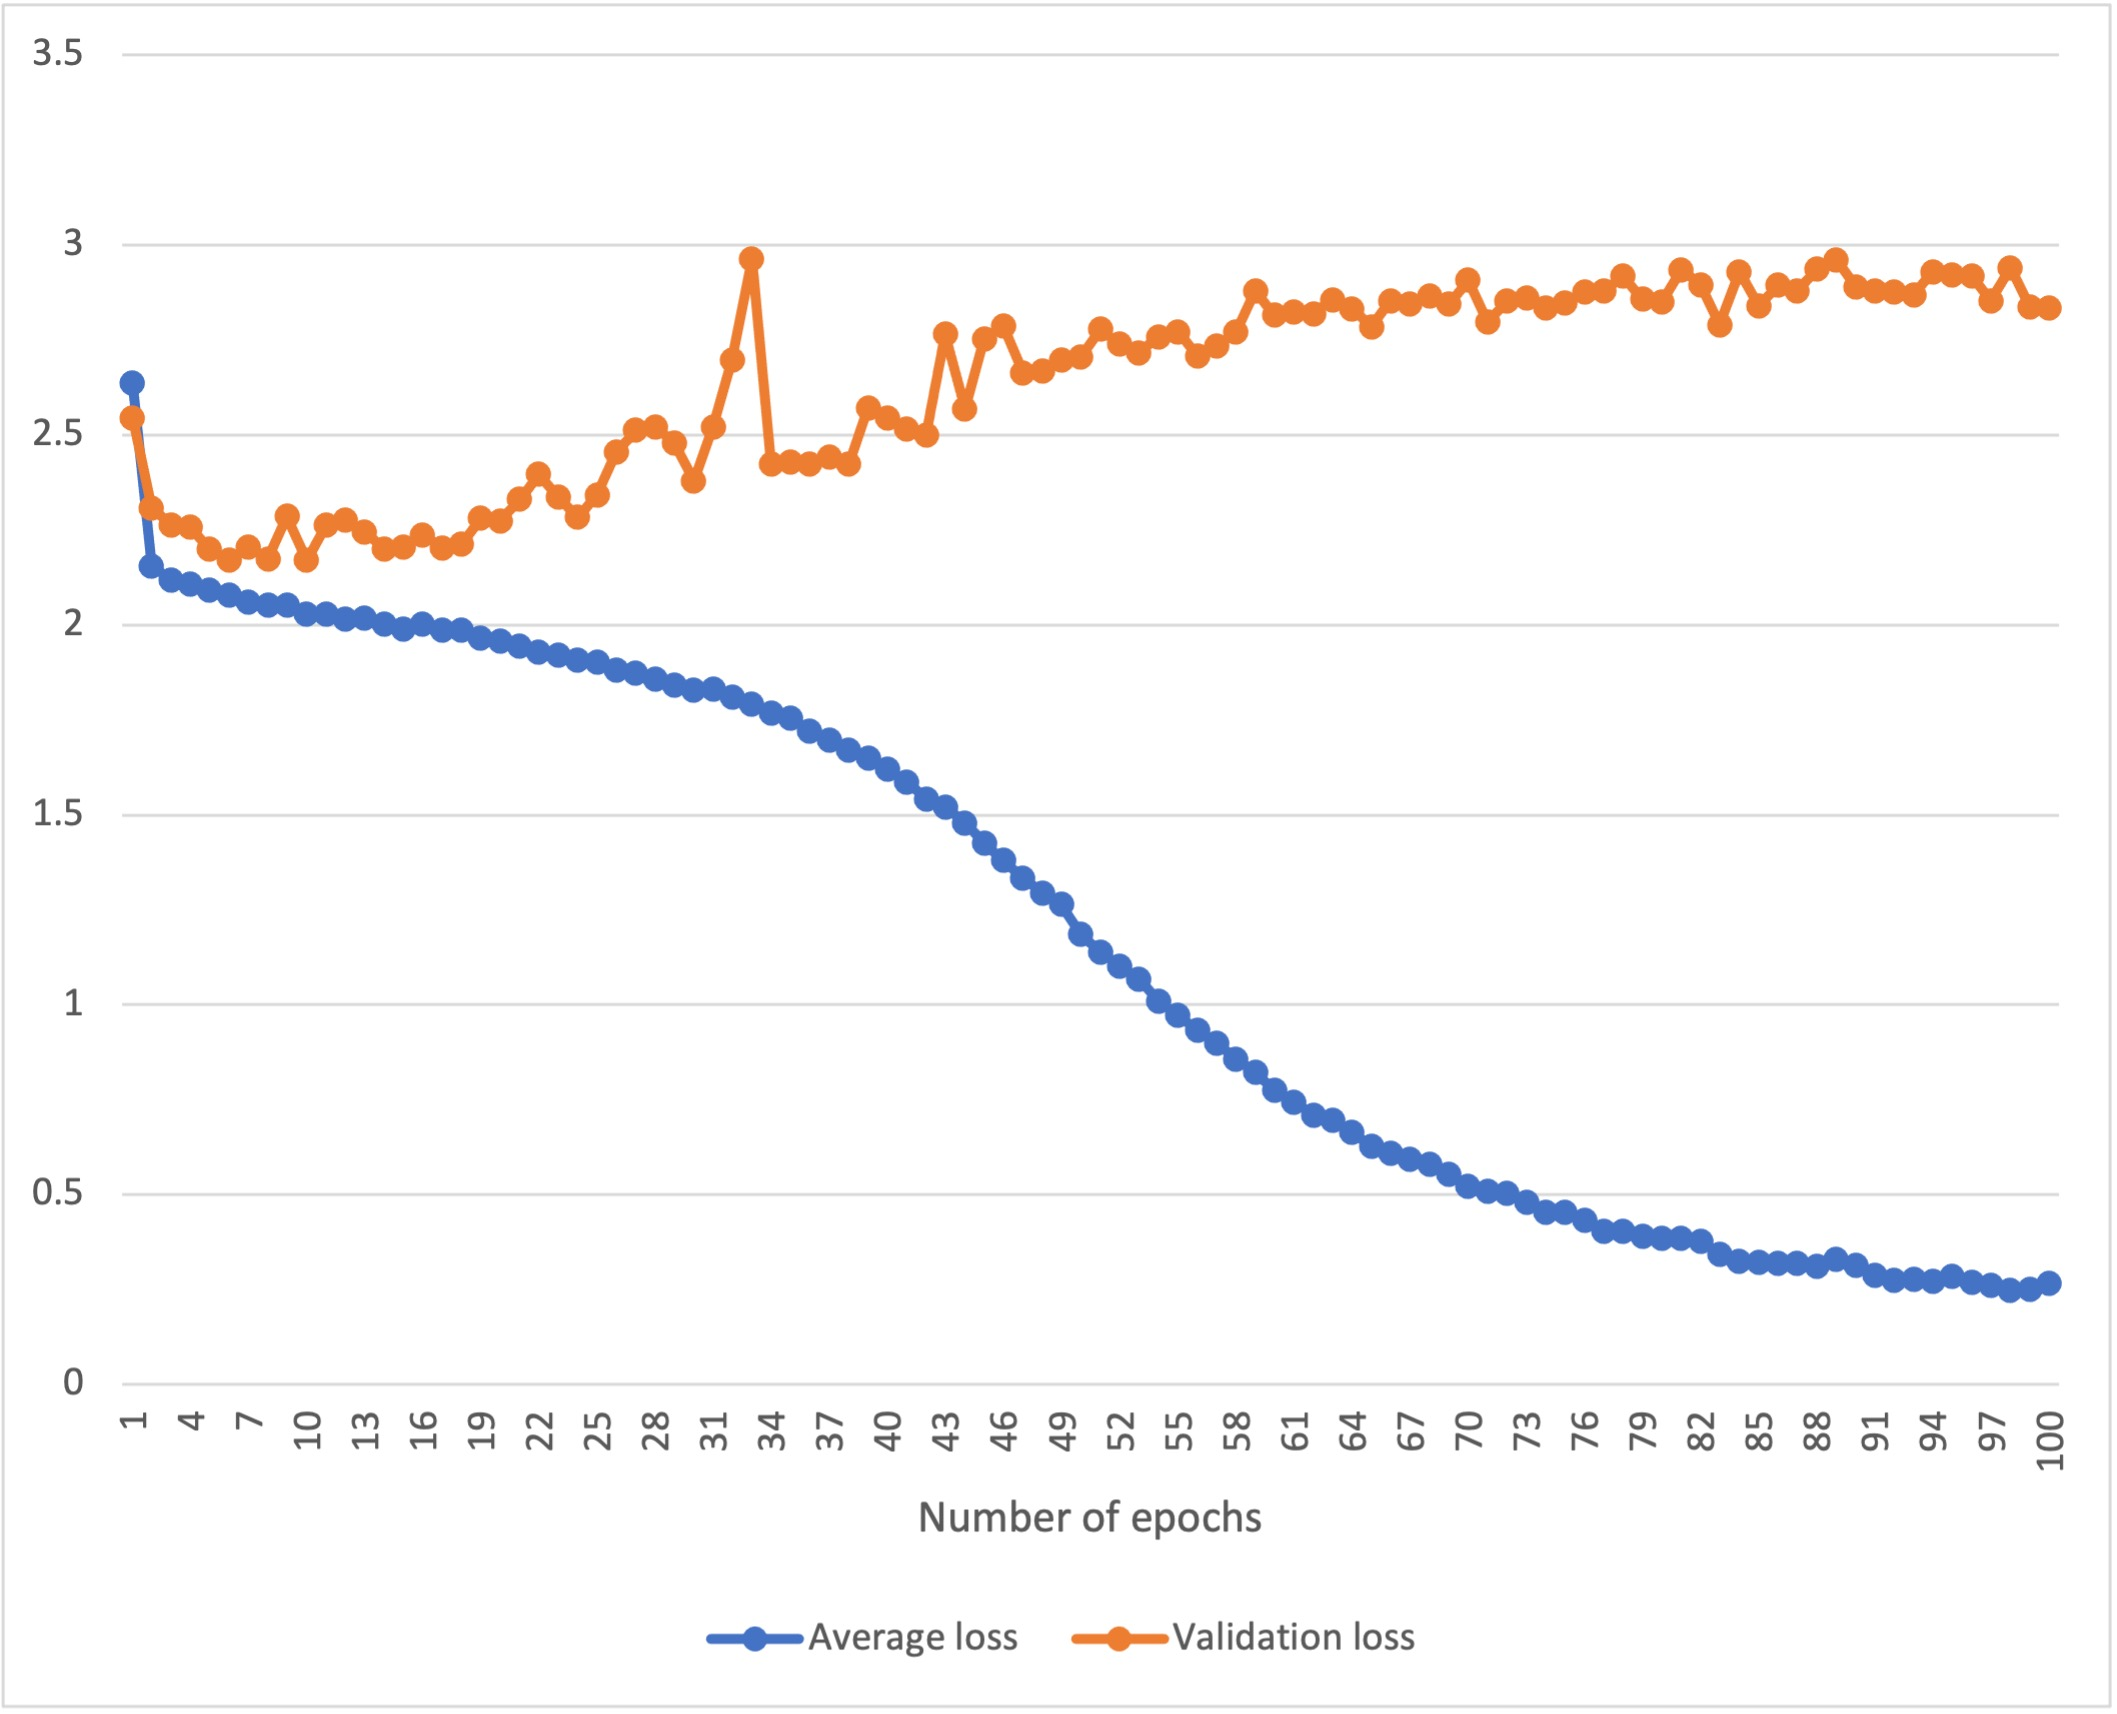
\includegraphics[width=3.5in]{images/epochgraph.jpg}\\
 \caption{YOLOv3 model accuracy and loss by number of training epochs \cite{radiology_error}.}\label{fig:compare}
 \end{center}
\end{figure}

% =======
% FIG. 04
% =======
\begin{figure}
 \begin{center}
 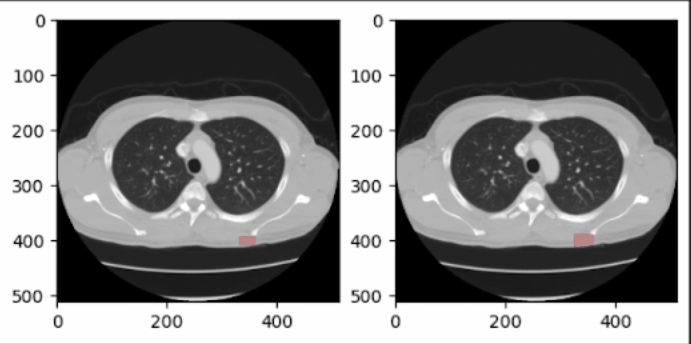
\includegraphics[width=3.5in]{images/training performance.PNG}\\
 \caption{Bounding box predictions for an image from the training set. The left image shows the model's output and the right shows the ground truth.}\label{fig:training}
 \end{center}
\end{figure}

% =======
% FIG. 05
% =======
\begin{figure}
 \begin{center}
 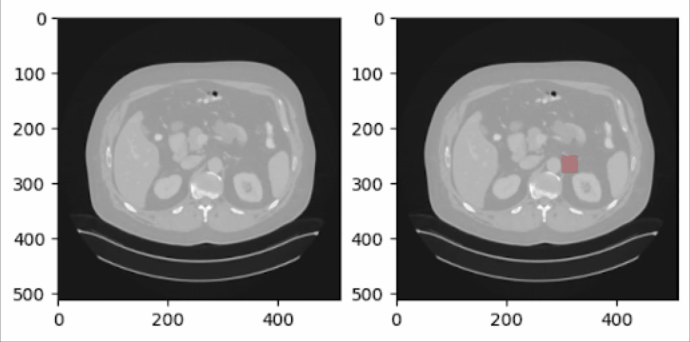
\includegraphics[width=3.5in]{images/testing performance.png}\\
 \caption{Bounding box predictions for an image from the testing set. The model failed to make any predictions on the new image.}\label{fig:testing}
 \end{center}
\end{figure}

% === VI. DISCUSSION ========================
% =================================================================================
\section{Discussion}
\subsection{Implementation challenges}
Progress was greatly impeded by the high barrier to entry of Deep Learning frameworks. We initially attempted to build the model in TensorFlow, but its lack of native GPU support for Windows motivated us to migrate to Pytorch. 

Setting up the code framework and data preprocessing pipeline took a deceptively long time. It took so long that we nearly ran out of time to implement the YOLOv3 model, and we didn't have enough time to tinker with the model further and explore using the entire DeepLesion dataset for training. Future projects should take into account the amount of time data preprocessing will take and plan accordingly by dedicating lots of time to it.

The first model was a quickly thrown together CNN as a placeholder to make sure the core elements of the code were working properly. It was unable to sufficiently optimize the loss and either refused to make predictions at all, resulting in very low bounding box confidences for all grids, or alternatively it predicted all grids as having bounding boxes, with relatively high confidence for all of them. At this point, we decided to apply YOLOv3 to attempt to improve the results.

\subsection{Future work}
Future research in this area should focus on applying additional models to compare performance, including some pre-trained models such as UNet \cite{unet}, as well as training on the full DeepLesion dataset to improve the performance of the current model, as we were only able to train on the Kaggle subset due to computational limitations \cite{kaggle}. Furthermore, To ensure that the data is not potentially skewed based on the anatomic differences of individual patients, we can split the records by patient when performing the train-test-validation split \cite{chollet_deep_learning}. 

Additionally, it would be beneficial to address the possibility of skewed data due to all images in the dataset containing a lesion, and some lesions not being annotated \cite{deeplesion}. A possible solution that is more accessible is to remove lesions for part of the data, either by slicing out part of the image entirely or by using content-aware filling, such that our model will not be biased towards always predicting lesions on scans. On the other hand, a more accurate solution is to employ additional expert annotation on the existing data, but given the size of the dataset, this would be extremely resource-intensive. Unsupervised learning approaches could also be considered, and compared with current findings.


\section*{Team Reflection}
All three of the authors have a background in computer science and not biology. As such, our focus was on processing the data and implementing AI models with high accuracy, and not on the underlying biological significance of lesions.

\bibliographystyle{IEEEtran}
\bibliography{IEEEabrv,Bibliography}

\vfill
\end{document}

% An example of a floating figure using the graphicx package.
% Note that \label must occur AFTER (or within) \caption.
% For figures, \caption should occur after the \includegraphics.
% Note that IEEEtran v1.7 and later has special internal code that
% is designed to preserve the operation of \label within \caption
% even when the captionsoff option is in effect. However, because
% of issues like this, it may be the safest practice to put all your
% \label just after \caption rather than within \caption{}.
%
% Reminder: the "draftcls" or "draftclsnofoot", not "draft", class
% option should be used if it is desired that the figures are to be
% displayed while in draft mode.
%
%\begin{figure}[!t]
%\centering
%\includegraphics[width=2.5in]{myfigure}
% where an .eps filename suffix will be assumed under latex, 
% and a .pdf suffix will be assumed for pdflatex; or what has been declared
% via \DeclareGraphicsExtensions.
%\caption{Simulation Results}
%\label{fig_sim}
%\end{figure}

% Note that IEEE typically puts floats only at the top, even when this
% results in a large percentage of a column being occupied by floats.


% An example of a double column floating figure using two subfigures.
% (The subfig.sty package must be loaded for this to work.)
% The subfigure \label commands are set within each subfloat command, the
% \label for the overall figure must come after \caption.
% \hfil must be used as a separator to get equal spacing.
% The subfigure.sty package works much the same way, except \subfigure is
% used instead of \subfloat.
%
%\begin{figure*}[!t]
%\centerline{\subfloat[Case I]\includegraphics[width=2.5in]{subfigcase1}%
%\label{fig_first_case}}
%\hfil
%\subfloat[Case II]{\includegraphics[width=2.5in]{subfigcase2}%
%\label{fig_second_case}}}
%\caption{Simulation results}
%\label{fig_sim}
%\end{figure*}
%
% Note that often IEEE papers with subfigures do not employ subfigure
% captions (using the optional argument to \subfloat), but instead will
% reference/describe all of them (a), (b), etc., within the main caption.


% An example of a floating table. Note that, for IEEE style tables, the 
% \caption command should come BEFORE the table. Table text will default to
% \footnotesize as IEEE normally uses this smaller font for tables.
% The \label must come after \caption as always.
%
%\begin{table}[!t]
%% increase table row spacing, adjust to taste
%\renewcommand{\arraystretch}{1.3}
% if using array.sty, it might be a good idea to tweak the value of
% \extrarowheight as needed to properly center the text within the cells
%\caption{An Example of a Table}
%\label{table_example}
%\centering
%% Some packages, such as MDW tools, offer better commands for making tables
%% than the plain LaTeX2e tabular which is used here.
%\begin{tabular}{|c||c|}
%\hline
%One & Two\\
%\hline
%Three & Four\\
%\hline
%\end{tabular}
%\end{table}


% Note that IEEE does not put floats in the very first column - or typically
% anywhere on the first page for that matter. Also, in-text middle ("here")
% positioning is not used. Most IEEE journals use top floats exclusively.
% Note that, LaTeX2e, unlike IEEE journals, places footnotes above bottom
% floats. This can be corrected via the \fnbelowfloat command of the
% stfloats package.


